\chapter{\texorpdfstring{P and NP}{P and NP}}
\label{ch:17aux}
\lecturemeta{Lezione 17aux \quad\textbullet\quad 2026-07-04 \quad\textbullet\quad Roberto Bruni}{Computational complexity (materiale ausiliario)}

Questa è una \textbf{lezione ausiliaria}: un ripasso di teoria della complessità che ci serve come sfondo per capire \emph{quanto costa} verificare le proprietà dei Petri net. Molte domande sulle reti (raggiungibilità, soundness, liveness) sono computazionalmente difficili, e per parlarne con precisione servono le classi \textbf{P} e \textbf{NP}. L'obiettivo qui è solo fissare il vocabolario.

\section{\texorpdfstring{Problemi, istanze, problemi di decisione}{Problemi, istanze, problemi di decisione}}

Prima di parlare di difficoltà, distinguiamo bene tre cose.

\begin{boxdefinition}{Problema, istanza, problema di decisione}
\begin{itemize}
\item Un \textbf{problem} definisce una \emph{famiglia} di domande collegate. Es. il \emph{factorization problem}: «dato un numero $n$, restituisci tutti i suoi fattori primi».
\item Un \textbf{problem instance} è \emph{una singola} di quelle domande. Es. «restituisci i fattori primi di 18».
\item Un \textbf{decision problem} è un problema la cui risposta è solo \textbf{booleana} (sì/no). Es. «dato $n$, è primo?»; istanza: «18 è primo?».
\end{itemize}
\end{boxdefinition}

Le classi di complessità si definiscono sui \textbf{decision problem}. La \textbf{Computational Complexity Theory} studia le \emph{risorse} necessarie a risolverli: quante operazioni di base (\textbf{time}) o quanta memoria (\textbf{space}) servono, in funzione della \textbf{dimensione dell'input}.

\section{\texorpdfstring{La classe P: risolvibili in modo efficiente}{La classe P: risolvibili in modo efficiente}}

\begin{boxdefinition}{Classe P}
\textbf{P} è l'insieme dei decision problem risolvibili da un algoritmo \textbf{deterministico} in un numero di passi \textbf{polinomiale} rispetto alla dimensione dell'input.

Intuizione: i problemi in P si possono \textbf{risolvere effettivamente} (e, di conseguenza, anche verificare) — "polinomiale" è la nozione tecnica di \emph{trattabile}.
\end{boxdefinition}

Un esempio classico è il circuito euleriano.

\begin{boxexample}{Eulerian circuit (in P)}
«Dato un grafo $G$, esiste un \textbf{circuito euleriano}?» (un circuito che percorre \textbf{ogni arco esattamente una volta}).

Si dimostra che equivale a chiedere: «il \textbf{grado} di ogni vertice è \textbf{pari}?» — condizione controllabile in \textbf{tempo lineare} nel numero di archi. Quindi il problema si risolve effettivamente: sta in \textbf{P}.
\end{boxexample}

\section{\texorpdfstring{La classe NP: verificabili in modo efficiente}{La classe NP: verificabili in modo efficiente}}

\begin{boxdefinition}{Classe NP}
\textbf{NP} è l'insieme dei decision problem risolvibili da un algoritmo \textbf{non-deterministico} in tempo polinomiale.

Equivalentemente (e più utile da immaginare): NP è l'insieme dei problemi le cui \textbf{soluzioni si possono verificare} da un algoritmo deterministico in tempo polinomiale.

Intuizione: le soluzioni dei problemi in NP si possono \textbf{controllare effettivamente} — se qualcuno ti dà una candidata risposta, la sai validare in fretta, anche se \emph{trovarla} potrebbe essere costoso.
\end{boxdefinition}

L'esempio speculare all'euleriano è il circuito hamiltoniano — apparentemente simile, ma di tutt'altra difficoltà.

\begin{boxexample}{Hamiltonian circuit (in NP)}
«Dato un grafo $G$, esiste un \textbf{circuito hamiltoniano}?» (un circuito che \textbf{visita ogni vertice esattamente una volta}).

Se qualcuno ti \emph{propone} un circuito, verificare che sia hamiltoniano è facile (\textbf{checked effectively}). Ma \textbf{trovarlo} sembra difficile: non si conosce un algoritmo polinomiale. Il problema \textbf{sembra} difficile da risolvere, pur essendo facile da controllare.
\end{boxexample}

\begin{figure}[!htb]
\centering
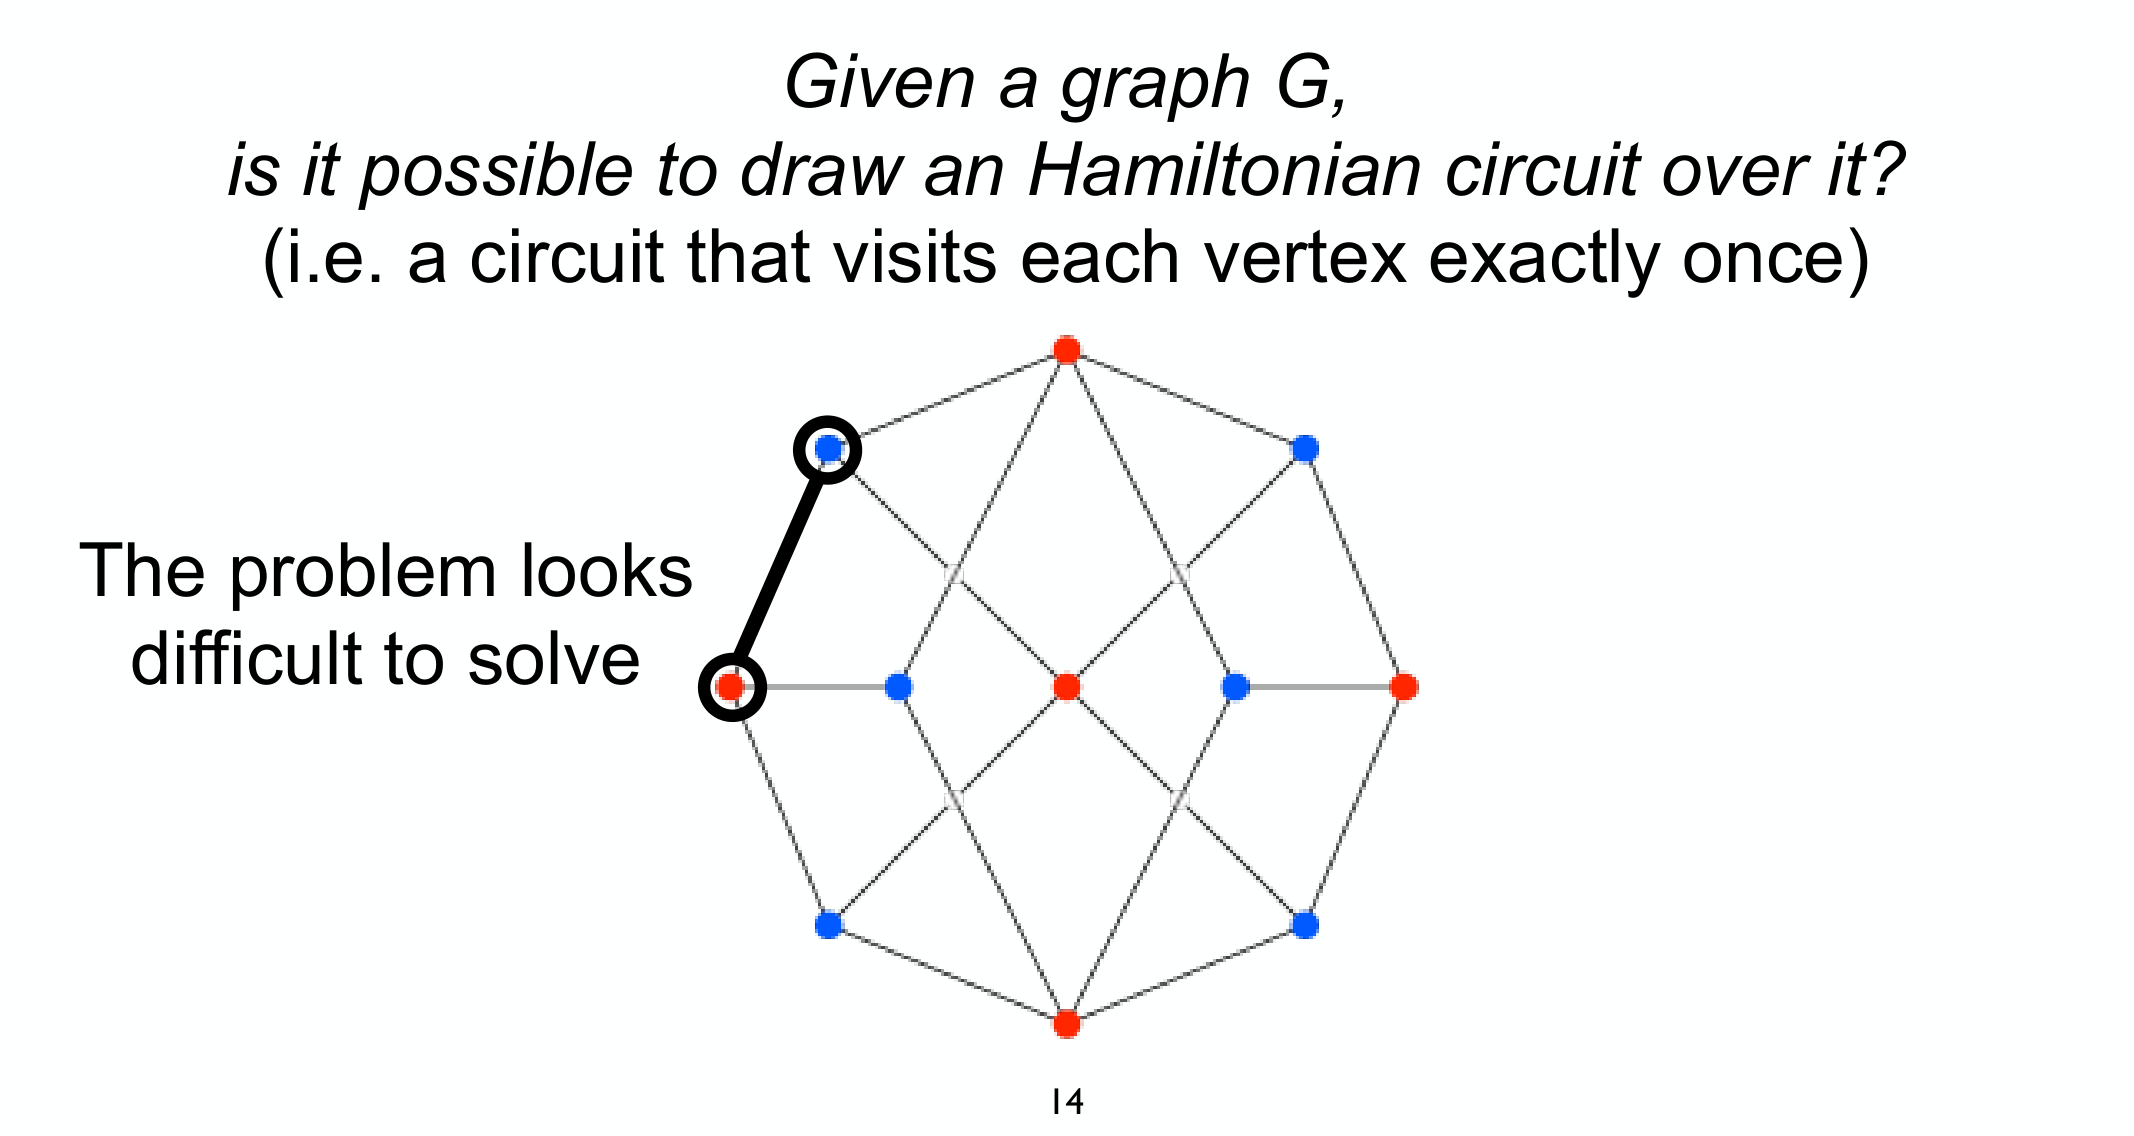
\includegraphics[width=0.74\linewidth,height=0.34\textheight,keepaspectratio]{images/17aux-p-np_p14_hamiltonian.png}
\caption{Hamiltonian circuit: verificare una soluzione data è immediato, ma costruirla richiede (per quanto si sa) di esplorare un numero enorme di combinazioni.}
\end{figure}

\begin{boxnote}{P $\subseteq$ NP}
Ogni problema in P sta anche in NP: se lo sai \emph{risolvere} in fretta, in particolare sai \emph{verificare} una soluzione in fretta (basta risolverlo e confrontare). Il viceversa è il grande interrogativo.
\end{boxnote}

\section{\texorpdfstring{Il problema P vs NP}{Il problema P vs NP}}

\begin{boxabstract}{La domanda da un milione di dollari}
Se \textbf{P = NP}, allora "risolvere" un problema non sarebbe più difficile che "controllarne" una soluzione. Se \textbf{P $\neq$ NP}, esistono problemi facili da verificare ma intrinsecamente difficili da risolvere.

\textbf{P = NP?} è la \textbf{più importante questione aperta} dell'informatica. La nostra esperienza quotidiana suggerisce che risolvere sia molto più arduo che verificare (correggere un compito è più facile che svolgerlo), da cui la congettura diffusa \textbf{P $\neq$ NP} — ma nessuno l'ha dimostrata.
\end{boxabstract}

\section{\texorpdfstring{NP-completeness e SAT}{NP-completeness e SAT}}

All'interno di NP ci sono i problemi "più difficili di tutti": gli \textbf{NP-complete}.

\begin{boxdefinition}{NP-completeness}
Un problema $Q \in$ NP è \textbf{NP-complete} se \textbf{ogni altro} problema in NP si può \textbf{ridurre} a $Q$ in tempo polinomiale.

Conseguenza: trovare un modo \emph{efficiente} di risolvere \textbf{un solo} problema NP-complete permetterebbe di risolvere efficientemente \textbf{tutti} i problemi in NP — cioè dimostrerebbe P = NP. Gli NP-complete sono quindi i candidati naturali per attaccare la domanda P vs NP.
\end{boxdefinition}

Il capostipite storico è \textbf{SAT}, la soddisfacibilità booleana.

\begin{boxdefinition}{SAT decision problem (NP-complete)}
Ingredienti: - \textbf{Variables}: un insieme di variabili booleane

\[
x_1, x_2, \dots, x_n
\]

\begin{itemize}
\item \textbf{Literals}: una variabile o la sua negazione
\end{itemize}

\[
x_i \quad \text{oppure} \quad \bar{x_i}
\]

\begin{itemize}
\item \textbf{Clause}: una \textbf{disgiunzione} di literal (un OR), es.
\end{itemize}

\[
(x_1 \vee \bar{x_3})
\]

\begin{itemize}
\item \textbf{Formula}: una \textbf{congiunzione} di clause (un AND di OR — forma normale congiuntiva).
\end{itemize}

Esempio:

\[
\varphi = (x_1 \vee \bar{x_3}) \wedge (x_1 \vee \bar{x_2} \vee x_3) \wedge (x_2 \vee \bar{x_3})
\]

\textbf{Domanda}: esiste un'assegnazione di valori booleani alle variabili tale che $\varphi = \text{true}$?

Per l'esempio, questa assegnazione funziona:

\[
x_1 = x_2 = x_3 = \text{true}
\]
\end{boxdefinition}

SAT è stato il \textbf{primo} problema dimostrato NP-complete (teorema di Cook–Levin): verificare un'assegnazione è banale, ma \emph{trovarne} una soddisfacente è, per quanto si sa, difficile.

Con questo vocabolario in mano, nella prossima lezione possiamo apprezzare perché i \textbf{free-choice net} sono così importanti: sono una classe per cui proprietà altrimenti costose diventano verificabili in modo trattabile. $\rightarrow$ \hyperref[ch:17]{17 — Free Choice}